\documentclass{article}
\usepackage{amsmath, amssymb, color, xcolor}
\usepackage{graphicx, wrapfig, float, caption, dsfont, bbm}
\usepackage{fullpage}
\usepackage[backref=page, hidelinks, colorlinks=true, citecolor=blue!60!black!100]{hyperref}
\usepackage{tikz}
\usetikzlibrary{arrows.meta, shapes}
\usepackage{caption, subcaption}
\usepackage{natbib} % gives us \citet: Author (year) and \citep: (Author; year)
\usepackage{authblk}

\usepackage{multicol}

\newcommand{\plr}[1]{{\color{blue}\it #1}}
\newcommand{\jss}[1]{{\color{olive}\it #1}}
% \newcommand{\ddt}{\frac{d}{dt}}
\newcommand{\ddt}{\dot}
\newcommand{\ro}{{ro}}
\newcommand{\nro}{{\bar{r}o}}
\newcommand{\rno}{{r\bar{o}}}
\newcommand{\nrno}{{\bar{r}\bar{o}}}
\newcommand{\reachable}{\mathcal{R}}
\newcommand{\unobservable}{\bar{\mathcal{O}}}
\newcommand{\R}{\mathbb{R}}
\newcommand{\E}{\mathbb{E}}
\renewcommand{\P}{\mathbb{P}}
\newcommand{\pda}{\frac{\partial}{\partial A_{ij}}}
\newcommand{\ind}{\mathds{1}}

\newcommand{\calA}{\mathcal{A}}
\newcommand{\calH}{\mathcal{H}}
\newcommand{\diag}{\text{diag}}
\newcommand{\1}{\mathbbm{1}}

\DeclareMathOperator{\spn}{span}

\newtheorem{theorem}{Theorem}
\newtheorem{lemma}{Lemma}
\newtheorem{definition}{Definition}
\newtheorem{example}{Example}

\begin{document}

\section*{The evolution of phenotypically invariant gene networks with implications for speciation, adaptation, and neutral variation}
{\centering
Joshua S. Schiffman$^{\dagger}$ \qquad Peter L. Ralph$^{\dagger \ddagger}$ \\
$^{\dagger}$University of Southern California, Los Angeles, California \qquad $^{\ddagger}$University of Oregon, Eugene, Oregon \\
\texttt{jsschiff@usc.edu} \qquad \texttt{plr@uoregon.edu}
\\
}

%\begin{multicols}{2}


\begin{abstract}
 % \textbf{
I will outline an analytical theory to study the evolution of biological systems such as gene regulatory networks, borrowing insight and tools from control engineering, systems identification, and dynamical systems theory. I will describe a null model of regulatory network evolution by analytically describing the set of all linear gene networks (of any size) that produce identical phenotypes -- and the evolutionary paths connecting them. In the idealized case of a perfectly adapted population, constant selection, and a static environment, we observe neutral evolution as a random walk over the phenotypically- invariant network-space. Under neutral conditions, this model can provide descriptions of expected network size and connectivity under mutation-selection equilibrium, estimate the rate of regulatory rewiring, and the rates at which Dobzhansky-Muller incompatibilities arise in reproductively isolated populations. This analysis provides insight into the mechanisms and parameters important for understanding developmental systems drift, network rewiring, evolvability, epistasis, and speciation, as well as the tenuous connection between network architecture and function. 
%}
\end{abstract}

Additional ideas to consider adding:
\begin{itemize}
    \item Haldane's rule (easy point in discussion: makes F1s look like F2s)
    \item add point about F1: quartic and F2: quadratic to results and maybe abstract/discussion
    \item hybrid vigor (need to do calculation)
    \item discuss linearity, linearization, and canalization in introduction
    \item obtain estimates of variation in $A$ from thermodynamic occupancy model
\end{itemize}

%%%%%%%%%%%%%%%%%%%%%%
\section*{Introduction}

Bridging the gulf between an organism's genome and phenotype is a poorly understood and complex molecular machinery. Progress in a suite of biological subdisciplines is stalled by our general lack of understanding of this molecular machinery: with respect to both its function and evolution. There does exist a growing body of experiment and data on the evolutionary histories and molecular characterizations of particular gene regulatory networks \citep{jaeger2011gap, davidson2006gene, israel2016comparative}, as well as thoughtful verbal and conceptual models \citep{true2001developmental, gwagner1, weiss2000phenogenetic, edelman2001degeneracy}. However, as Hardy and Weinberg taught us over a century ago, verbal theories are often insufficient, if not downright misleading \citep{hardy1908mendelian, weinberg1908vererbungsgesetze, servedio2014not}. This is especially pertinent given the staggering complexity and scope of contemporary research programs. This outlook necessitates the advancement of conceptual frameworks of such precision, only mathematics will suffice, as models allow the development of concrete numerical predictions. Previously it has been suggested that any idealized study of evolution is incomplete without a mathematically sufficient description of the genotype, phenotype, and transformation from one to the other \citep{Lewontin1974genetic}.%Here we outline an analytical theory to study the evolution of biological systems, borrowing insight and methods from control engineering, systems identification, and dynamical systems theory. 

%Presently, we focus on the neutral evolution of genetic regulatory networks. That is, we analytically describe the set of all linear gene networks (of any size) that produce identical phenotypes -- and the evolutionary paths connecting them. In the idealized case of a perfectly adapted population, constant selection, and a static environment, we observe evolution under the ``conservation of phenotype'' as a Brownian motion over phenotypically-invariant network-space. This analysis provides insight to the mechanisms and parameters important for understanding developmental systems drift, network rewiring, evolvability, epistasis, and speciation, as well as the tenuous connection between network architecture and function.


%It is commonly taught that an organism's genome contains the heritable material 
%that natural selection filters and that an organism's phenotype directly determines its
%evolutionary fitness. Between genotype and phenotype is an often complicated and poorly
%undrstood molecular machinery -- and it is a major goal common to many different disciplines
%within the life sciences to elucidate its form, function, and evolution. These aims are
%delicately intertwined and a comphrehensive understanding of a system's evolution requires
%an understanding of its function and vice versa.

The molecular machinery, interacting with the environment, and bridging genotype to phenotype
can be mathematically described as a dynamical system -- or a system of differential equations\citep{jaeger2015comet}.
 Movement in this direction is ongoing, as researchers have begun to study 
the evolution of both abstract \citep{wagner1994evolution, wagner1996does,  siegal2002waddington, bergman2003evolutionary, draghi2015robustness} and empirically inspired computational and mathematical models of gene regulatory networks (GRNs) \citep{mjolsness1991connectionist, jaeger2004dynamic, maria1, vitaly1, vitaly2, crombach2016gap, wotton2015quantitative, chertkova2017insilico}. If we allow the reasonable assumption that the genotype-phenotype map can be represented as a system of differential equations, we can immediately discuss its evolution and function in a much more mechanistic, yet general, manner. 

In some fields that seek to fit parametric models to experimental data, such as control
theory, chemical engineering, and statistics, it is well known that mathematical models
can fundamentally be \emph{unidentifiable} and/or \emph{indistinguishable} -- meaning that 
there can be uncertaintity about an inferred model's parameters or even its claims about
causal structure, even with access to complete and perfect data \citep{bellman1970structural, grewal1976identifiability, walter1984structural}. Models with different 
parameter schemes, or even different mechanics can be equally accurate, but still not
\emph{actually} agree with what is being modelled. In control theory, where electrical 
circuits and mechanical systems are often the focus, it is understood that there can be an 
infinite number of ``realizations'', or ways to reverse engineer the dynamics of a black box,
even if all possible input and output experiments on the black box are performed \citep{kalman1963mathematical, anderson1966equivalence, zadeh1976linear}. In chemical
engineering, those who study chemical reaction networks sometimes refer to the fundamental
unidentifiability of these networks as ``the fundamental dogma of chemical kinetics'' \citep{craciun2008identifiability}. In computer science, this is framed as the relationship among processes that simulate one another \citep{van2004equivalence}.
Although this may frusturate the occasional engineer or scientist, viewed from another angle,
the concepts of unidentifiability and indistinguishability can provide a starting point for
thinking about externally equivalent systems -- systems that evolution can explore, so long
as the parameters and structures can be realized biologically. In fact, evolutionary
biologists who study convergent versus parallel evolution, homology, and analogy are very familiar with such functional symmetries; macroscopically identical phenotypes in even very closely related species can in fact be divergent at the molecular and sequence level \citep{true2001developmental, tsong2006evolution, hare2008sepsid, vierstra2014mouse, stergachis2014conservation, taylor2016diverse, matsui2015regulatory}.

  In this paper we propose a framework to study the evolution of biological systems. We expect wide applicability to this approach (\emph{i.e.} non-neutral evolution), however presently, we focus solely on neutral evolution. To begin, we focus on the evolution of an idealized population. We consider the neutral evolution of a large population, evolving in a static environment. Under these circumstances we expect the population explores the manifold of phenotypically invariant (or symmetric) gene regulatory networks.

  Presently we ask two questions, (1) holding the phenotype and environment constant for evolutionary time, how much do we expect gene network organization to drift, and (2) does this contribute to speciation, primarily via the fixation of reproductive incompatibilities?

\section*{Gene Networks as Linear Dynamical Systems}

  \jss{Organisms' phenotypes are constructred by gene by gene by environment interactions. Here we simply define the phenotype to be the organismal temporal molecular dynamics directly under natural selection. The \emph{what}, \emph{when}, and \emph{where}, of an organism's molecules that are physiologically or otherwise relevant for survival. 
   Thus we say that some function $\phi(t)$ is a phenotype where, 
  \begin{align}
    \phi(t) = \int_{0}^{\infty} h(t) u(t) dt  ,
  \end{align}
  and $h(t)$ is the \emph{impulse response} of the system and $u(t)$ is the \emph{input} function, both functions of time $t$. The input can be interpreted as the environment, as initial conditions, or otherwise, depending on the biological specifics under study. The phenotype is a convolution of both the impulse response and the input, as allowed by our assumption of linearity. 

  Essentially the phenotype $\phi(t)$ is a consequence of an organism's specific gene by gene interactions, given by $h(t)$, reacting further with the local environment, given by $u(t)$. 

  We describe the impulse response as, 
  \begin{align}
    h(t) = C e^{A t} B
  \end{align}
  where $A$ is a gene regulatory network (although this model can be generalized to other biological networks) -- a square matrix, and $B$ filters and translates the input to the system. The form of $B$ determines precisely how the state of the external environment influences the internal gene network. $C$ filters and translates the dynamics of the system and precesily determines the output, that is, what is visible to selection. 

  Generally $A$ can be any real $n \times n$ matrix, $B$ any $n \times \ell$, and $C$ any $\ell \times n$ dimensional matrix. Each $i$th row of $A$ describes the \emph{cis}-regulatory module for gene $i$, and each $j$th entry, the specific regulatory influence of gene $j$ on gene $i$. 

  Although $\phi(t)$ describes the phenotype given an input, $h(t)$ describes the phenotype subject only to an impulse -- an input present initially and absent immediately thereafter. Typically, a system $\Sigma$, is defined as,
  \begin{align}
    \Sigma = \left\{ \begin{array}{ll} \dot{\kappa}(t) &= A \kappa(t) + B u(t) \\ \phi(t) &= C \kappa(t) \end{array} \right.
  \end{align}
  Variables have the same identities as described above and $\kappa(t)$ is a vector of molecule concentrations at time $t$. Therefore the molecular concentrations at a specific time are completely determined by the input and gene by gene interactions. Lastly, a portion and/or combination of these molecules, $\phi(t)$, are ``observed'' by selection (this is in constrast to $\kappa(t)$ -- the \emph{kryptotype} -- as it is ``hidden'' from direct selection).
}

We will now lay out the model in more general terms.
Suppose that the \emph{internal state} of the system
is parameterized by the concentrations of a collection of $n$ molecular species,
$S_1, \ldots, S_n$,
and the vector of concentrations at time $t$ we denote $\kappa(t)=(\kappa_1(t),\ldots,\kappa_n(t))$.
There are also $m$ ``input'' species, whose concentrations are determined
exogenously to the system,
and are denoted $u(t) = (u_1(t),\ldots,u_m(t))$,
and $\ell$ ``output'' species, whose concentrations are denoted
$\phi(t) = (\phi_1(t),\ldots,\phi_\ell(t))$.
The output is merely a linear function of the internal state:
\begin{align*}
    \phi_i(t) = \sum_j C_{ij} \kappa_i(t).
\end{align*}
Since $\phi$ is what natural selection acts on, we refer to it as the \emph{phenotype},
and sometimes in contrast refer to $\kappa$ as the \emph{kryptotype},
as it is ``hidden'' from direct selection.
The rate at which the $i^\text{th}$ species is produced
is a weighted sum of the concentrations of the other species
as well as the input:
\begin{align*}
    \ddt \kappa_i(t) = \sum_j A_{ij} \kappa_j(t) + \sum_r B_{ir} u_r(t) .
\end{align*}
In matrix notation, this is written more concisely as
\begin{align} \label{eqn:lti_system}
    \ddt \kappa(t) &= A \kappa(t) + B u(t) \\
    \phi(t) &= C \kappa(t) .
\end{align}

  \begin{example}[Oscillating Gene Network: Cell Cycle Control]\label{ex:oscillator}


    Cellular division is a complicated phenomena, governed by many different processes, however it is agreed that its rhythm is partially controlled by periodic (oscillating) gene transcription \citep{orlando2008global}. Consider a simplified model of oscillating gene transcription. In the present framework periodic expression requires at minimum two interacting genes. 

    Suppose gene-2 up-regulates the transcription of gene-1 and that gene-1 down-regulates the transcription of gene-2 with equal magnitude (of $1$) and relative to each of their concentrations, denoted by $\kappa_{1}$ and $\kappa_{2}$. Furthermore, suppose that only the dynamics of gene-1 are consequential to the cell cycle (perhaps the amount of gene-1 activates another downstream gene network). Lastly suppose that the production of both genes is stimulated by an impulse of a molecule present immediately after division.

    If the rate each of these genes is expressed is a linear function of their concentrations, the dynamics of the system are given by
    \begin{align*}
      \dot{\kappa_{1}}(t) &= \kappa_{2}(t) + u(t) \\
      \dot{\kappa_{2}}(t) &= - \kappa_{1}(t) + u(t)
    \end{align*}
    where $\dot{\kappa}$ denotes the time derivative. The initial conditions $\kappa_{1}(0)$ and $\kappa_{2}(0)$, and the input $u(t)$ then determiine the concentrations through time. If we record the regulatory coefficients in the matrix
    \begin{align*}
      A &= \begin{bmatrix} 0 & 1 \\ -1 & 0 \end{bmatrix} ,
    \end{align*}
    and define the column vector $B = \begin{bmatrix} 1 & 1 \end{bmatrix}^{T}$, then in matrix notation the dynamics are
      \begin{align*}
      \dot{\kappa} &= A \kappa(t) + B u(t) .
      \end{align*}
      Since only the dynamics of gene-1 are directly relevant to biological function, the dynamics of interest are given by
      \begin{align*}
      \phi(t) &= C \kappa (t)
      \end{align*}
      where the row vector $C$ is defined as $C = \begin{bmatrix} 1 & 0 \end{bmatrix}$. (Note: if the dynamics of both genes were physiologically relevant to the cell cycle, we would set $C$ to be the identity matrix).
  %  \begin{align*}
  %    A = \begin{bmatrix} 0 & 1 \\ -1 & 0 \end{bmatrix} , \qquad B = \begin{bmatrix} 1 \\ 1 \end{bmatrix}, \qquad C = \begin{bmatrix} 1 & 0 \end{bmatrix}
  %  \end{align*}
 %       The oscillatory system $\Sigma$ is thus given as
 %   \begin{align*}
 %     \Sigma = \left \{ \begin{array}{ll} \dot{\kappa}(t) &= \begin{bmatrix} 
 %       0 & 1 \\ 
 %      -1 & 0 
 %       \end{bmatrix} \kappa(t) + \begin{bmatrix} 1 \\ 1 \end{bmatrix} u(t) \\ 
 %         \phi(t) &= \begin{bmatrix} 1 & 0 \end{bmatrix} \kappa(t) \end{array} \right.
 %    \end{align*}
      
      Since the input is simply an impulse, its phenotype is equivlanet to its impulse response

      \begin{align*}
        \phi(t) = h(t) = \sin(t) + \cos(t)  .
      \end{align*}

    \begin{figure}[H]
       % \begin{center} 
      \centering
         \begin{tabular}{cc}
            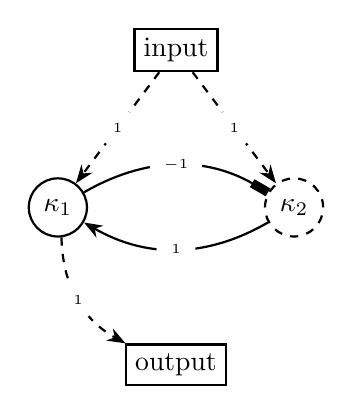
\begin{tikzpicture}
            \begin{scope}[every node/.style={circle,thick,draw}]
                \node (A) at (0,0) {$\kappa_{1}$};
                \node[dashed] (B) at (3,0) {$\kappa_{2}$};
                \node[shape=rectangle] (U) at (1.5,2) {input};
                \node[shape=rectangle] (y) at (1.5,-2) {output};
            \end{scope}

            \begin{scope}[>={Stealth[black]},
                          every node/.style={fill=white,circle},
                          every edge/.style={draw=black, thick}]
                \path [->, >=Rectangle] (A) edge[bend left] node {\tiny $-1$} (B);
                \path [->] (B) edge[bend left] node {\tiny $1$} (A); 
                \path[->] (U) edge[dashed] node {\tiny $1$} (A);
                \path[->] (U) edge[dashed] node {\tiny $1$} (B);
                \path[->] (A) edge[dashed,bend right] node {\tiny $1$} (y);
            \end{scope}
            \begin{scope}[>={Stealth[black]},
                          every edge/.style={draw=black, thick}]
                %\path [->] (A) edge[loop left] node {\tiny $\lambda_{1}$} (A);
                %\path [->] (B) edge[loop left] node {\tiny $\lambda_{2}$} (B);
            \end{scope}

            \end{tikzpicture} &
       % \end{center}
      %  \caption{
      %      Diagram of Example \ref{ex:osc} in the text.
      %      \plr{explain what arrows mean if nec}
      %      \label{fig:oscillator_diagram}}
   % \end{figure}
   % \begin{figure}[H]
    %  \centering
      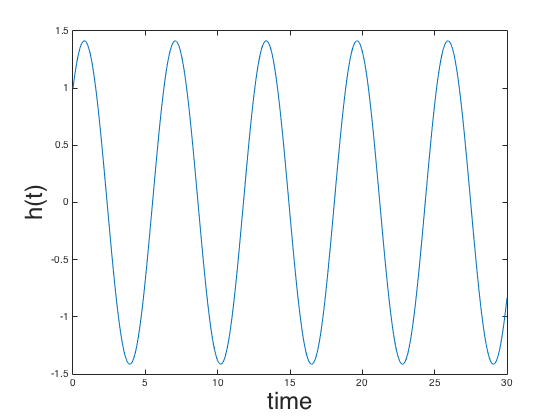
\includegraphics[width=0.5\textwidth, height=0.25\paperheight]{osc_impulse}
   \end{tabular}
  %  \end{center}
      \caption{(Left) Graphical representation of the cell cycle control gene network, and (right) plot of the phenotype $\phi(t)$ against time $t$.}
    \end{figure}
      We return to the evolution of such a system below.
  \end{example}

  \section*{The Model II: Linear Evolutionary Systems}

  The literature is filled with detailed observations of molecular systems and their diversity. There are examples of significant diversity in the networks underlying processes such as circadian rhythm \citep{sancar2008intelligent}, cell cycle control \citep{cross2011evolution, kearsey2003enigmatic}, pattern formation, and metabolism  \citep{lavoie2009rearrangements, martchenko2007transcriptional, dalal2016transcriptional, christensen2011unique, hartl2007induction, alam2013aspergillus}. Despite a symmetry in functionality or phenotype these systems often differ, sometimes substationaly, at the molecular level. How many different mechanisms have the same function? We urge the reader to consider the metaphorical black box.

  Systems with identical external dynamics do not necessarily have identical internal dynamics. Any linear and minimal system -- minimal, informally meaning that the system's external dynamics are achieved with the fewest possible number of internal components -- has identical external dynamics up to a change of coordinates. 
  \begin{align}
    h(t) &= C e^{A t} B \\
    &= C V^{-1} V e^{A t} V^{-1} V B \\
    &= C V^{-1} e^{V A V^{-1} t} V B \\
    &= \bar{C} e^{\bar{A} t} \bar{B}
  \end{align}
  Two systems, $\Sigma = \{ A, B, C \}$, and $\bar{\Sigma} = \{\bar{A} = VAV^{-1}, \bar{B} = VB, \bar{C} = CV^{-1} \}$, have the same dynamics if they are related by a change of coordinates. 

  Although systems may not be identifiable beyond a change of coordinates, at present we are primarily interested in a subset of these systems. That is, systems that not only have equivalent external dynamics, but also equivalent input and output relationships. Formally, this means systems related by a change of coordinates (any invertible matrix $V$) that leaves $B$ and $C$ invariant:
  \begin{align}
    VB &= B \implies \bar{B} = B \\
    CV &= C \implies \bar{C} = C
  \end{align}
  In other words systems with varying genetic architectures yet identical selection pressures, environment, and phenotype. 

  Define $V(\tau)$ as the parameterized change of coordinates matrix that preserves $B$ and $C$, with $\tau$ a vector of free parameters. The set of \emph{all} phenotypically invariant (minimal) gene networks is, 
  \begin{align}
    A(\tau) = V(\tau) A(0) V^{-1}(\tau) ,
  \end{align}
  and a \emph{Linear Evolutionary System} is, 
  \begin{align}
    \Sigma(\tau) = \left\{ \begin{array}{ll} \dot{\kappa}(t) &= A(\tau) \kappa(t) + B u(t) \\ \phi(t) &= C \kappa(t) \end{array} \right .
  \end{align}
  That is, all (linear and minimal) mechanisms capable of producing the same phenotype can be realized by a unique choice of $\tau$ in $\Sigma(\tau)$.

  More generally, \plr{introduce Kalman},
  we denote by $\calA_n(A_0)$ the set of all $n$-dimensional systems equivalent to $A_0$:
  \begin{equation} \label{eqn:equivalence}
      \begin{aligned}
      \calA_n(A_0) 
          &= \left\{
              A : C e^{At} B = C e^{A_0 t} B \; \text{for}\; t \ge 0 
          \right\}  \\
          &= \left\{
              A : C A^k B = C A_0^k B \; \text{for}\; 1 \le k \le n-1 
          \right\} .
      \end{aligned}
  \end{equation}
  Equivalence of the two characterizations follows from the Cayley-Hamilton theorem.
  Usually, the dimension $n$ and the reference system $A_0$ is implicit and we write only $\calA$.

  \begin{example}[All Phenotypically Equivalent Cell Cycle Control Networks]

    Let
    \begin{align*}
      A(0) = \begin{bmatrix} 0 & 1 \\ -1 & 0 \end{bmatrix}, \qquad B = \begin{bmatrix} 1 & 1 \end{bmatrix}^{T}, \qquad C = \begin{bmatrix} 1 & 0 \end{bmatrix},
    \end{align*}
    with $V(\tau)$ preserving both $B$ and $C$, then
    the set of all two-gene regulatory networks phenotypically equivalent to the cell cycle control network in Example \ref{ex:oscillator} are given by
    \begin{align*}
      A(\tau) &= \begin{bmatrix} 1 & 0 \\ \tau & 1-\tau \end{bmatrix} \begin{bmatrix} 0 & 1 \\ -1 & 0 \end{bmatrix} \begin{bmatrix} 1 & 0 \\ \frac{\tau}{\tau-1} & \frac{-1}{\tau-1} \end{bmatrix}  \qquad \forall \ \tau \neq 1 %\\
     %   B &= \begin{bmatrix} 1 \\ 1 \end{bmatrix}, \qquad C = \begin{bmatrix} 1 & 0 \end{bmatrix} \\
       %   h(t) &= \sin(t) + \cos(t) \qquad \forall \ \tau \neq 1
    \end{align*}
    \begin{figure}[H]
    \centering
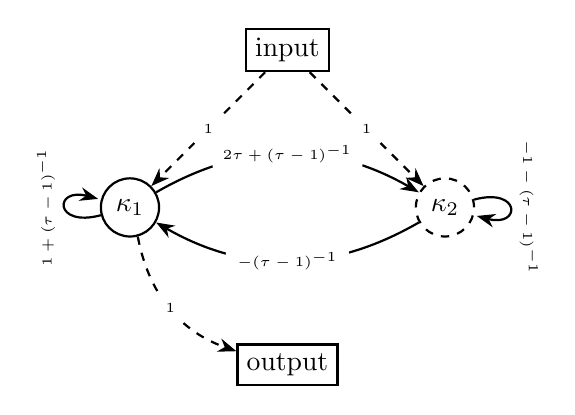
\begin{tikzpicture}
\begin{scope}[every node/.style={circle,thick,draw}]
  \node (A) at (0,0) {$\kappa_{1}$};
    \node[dashed] (B) at (4,0) {$\kappa_{2}$};
    \node[shape=rectangle] (U) at (2,2) {input};
    \node[shape=rectangle] (y) at (2,-2) {output};
\end{scope}

\begin{scope}[>={Stealth[black]},
              every node/.style={fill=white,circle},
              every edge/.style={draw=black, thick}]
    \path [->, sloped] (A) edge[bend left] node {\tiny $2 \tau + (\tau-1)^{-1}$} (B);
    \path [->, sloped] (B) edge[bend left] node {\tiny $-(\tau-1)^{-1}$} (A); 
    \path[->] (U) edge[dashed] node {\tiny $1$} (A);
    \path[->] (U) edge[dashed] node {\tiny $1$} (B);
    \path[->] (A) edge[dashed, bend right] node {\tiny $1$} (y);
\end{scope}
\begin{scope}[>={Stealth[black]},
              every edge/.style={draw=black, thick}]
    \path [->] (A) edge[loop left] node[sloped, anchor=center, above] {\tiny $1 + (\tau-1)^{-1}$} (A);
    \path [->] (B) edge[loop right] node[sloped, anchor=center, above] {\tiny $-1 - (\tau-1)^{-1}$} (B);
\end{scope}

\end{tikzpicture}
    \caption{A graphical depiction of the set of all externally equivalent cell cycle control networks, $A(\tau)$. $\tau$ can take any valye}
    \end{figure}
 % \end{example}

 % \begin{example}[External Equivalence does not imply internal equivalence]
   Despite the phenotypic equivalence of all instantiations of $A(\tau)$, the internal dynamics, or kryptotypes, vary as a function of $\tau$. 
    Gene-1 dynamics (blue) are equivalent for network architectures $A(0)$ and $A(2)$, however the dynamics of gene-2 (orange) differ with $\tau$.
  \begin{figure}[H]
    \centering
    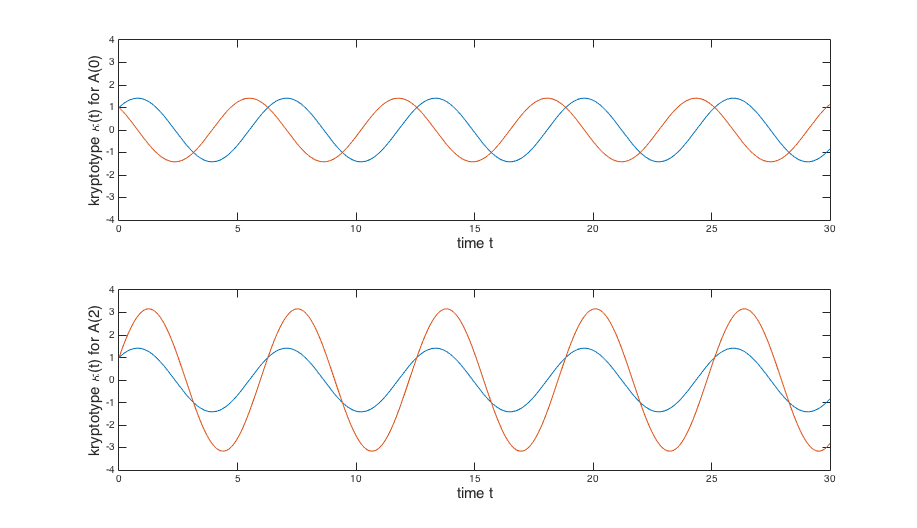
\includegraphics[width=0.5\textwidth, height=0.25\paperheight]{osc_A0_A2_both_compare}
    \caption{Gene-1 (blue) and gene-2 (orange) dynamics for $A(0)$ (top) and $A(2)$ (bottom). Both (top and bottom) gene-1 dynamics are given by $ \kappa_{1} = \sin(t) + \cos(t)$, and gene-2 by $\kappa_{2} = \cos(t) - \sin(t)$ (top) and $\kappa'_{2} = \cos(t) + 3 \sin(t)$ (bottom).}
  \end{figure}
  \end{example}

  %%%%%%%%%%%%%%%%%%%%%%%%
  \section*{Intraspecific variation and genetic drift}

  \plr{rework this: we assume optimal phenotype is fixed and population is large but polymorphic and not strictly on the optimum}

First we focus on a simple evolutionary scenario -- \emph{phenotypically invariant evolution}: a large population, perfectly adapted, and in a constant environment. In this circumstance we expect phenotype to be conserved throughout evolutionary time. As such we should only expect the phenotype to change as a consequence of genetic drift (small effective population size), adaptation to new selective and/or environemental pressures. These phenotypic variations should yield distinct signatures. Adaptative changes will change the optimal impulse response function $h(t) \xrightarrow{adaptation} h'(t)$. Genetic drift registers as an increase in the intrapopulation variation in $h(t)$. 
 \jss{added the phenotypic invariance stuff here (above) -- not sure if it should put elsewhere yet}

  At any given time, there will be a range of network coefficients present in the population
  due to segregating genetic polymorphism.
  Over many generations, even if selective pressures do not change,
  this range of networks will shift 
  as recombination, mutation, and demographic noise create new alleles and shift allele frequencies.
  How much variation do we expect to find within a population?
  Is this range limited by available variation or kept in check by selection?
  How fast will a population explore the space of equivalent networks?
  To answer these questions, we need to know two things known at best only roughly \citep{felsenstein1988phylogenies} --
  the strength of stabilizing selection on the phenotype,
  and the amount (and structure) of heritable variation in the genotype.
  We aim to get order-of-magnitude estimates.

  \plr{amount of heritable variation}
  We quantify (roughly) the amount of heritable variation
  by $\sigma^2$, the genetic variance present in a population in a typical entry of $A$.
  The coefficient $A_{ij}$ measures how much the rate of net production of $i$ changes
  per change in concentration of $j$.
  It is generally thought that regulatory sequence change contributes much more to inter- and intraspecific variation
  than does coding sequence change affecting molecular structure \citep{schmidt2010vertebrate}.
  In the context of transcription factor networks this may be affected 
  not only by the binding strength of $j$ to the promoter region of $i$
  but also the effects of other transcription factors (e.g., cooperativity)
  and local chromatin accessibliity \citep{stefflova2013cooperativity}.
  For this reason, 
  the mutational target size for variation in $A_{ij}$ may be much larger than the dozens of base pairs
  typically implicated in the handful of binding sites for transcription factor $j$ of a typical promoter region.
  (Recall that although these are best modeled through nonlinear terms,
  by linearizing we essentially consider first-order effects.)
  On the other hand, a diverse set of buffering mechanisms are thought to contribute to phenotypic stability
  in the presence of substantial molecular noise \citep{canalization,buffering},
  suggesting that substantial variation in the micro-scale dynamics we consider here
  may be necessary to produce relevant phenotypic effects downstream.
  \plr{replace "micro-scale" with sthg else or discuss earlier}
  Differences in $A_{ij}$ due to a sequence change are hard to measure 
  -- the closest available data we could find either related to variation in transcription factor binding site occupancy
  or in expression levels (e.g., cis-eQTL).
  The former may be an overestimate, 
  since it does not capture buffering effects (if for instance only one site of many needs be occupied for transcription to begin)
  and the latter probably measures changes in steady-state concentration (our $x_i$) rather than the rate of change.
  \citet{kasowski2010variation} found differential occupancy in 7.5\%
  of binding sites of a transcription factor (p65) between human individuals.
  \citet{verlaan2009targeted} showed that cis-regulatory variation
  accounts for around 2--6\% of expression variation in human blood-derived primary cells,
  while \citep{lappalainen2013transcriptome} found that human population variation 
  explained about 3\% of expression variation.
  \plr{Get some data from at least one other species in here!}
  Taken together, this suggests that variation in the entries of $A$
  may be on the scale of 1\% between individuals of a population --
  doubtless varying substantially between species and between genes.

  \plr{merge this above}
  The amount and structure of this standing variation is established over long time scales
  by many factors, including
  mutation-selection balance, 
  shifts in the phenotypic optimum,
  and/or spatial variation in the optimum \citep{hansen1996translating}.
  Quantitative genetics models of mutation-selection balance 
  predict precise levels and structure of standing variation \citep{kimura_mutsel,lande_mutsel,lande1981models},
  but it is unclear how well these predictions match reality \citep{johnson_barton}
  and how much they are expected to change over time \citep{arnold_changing_G}.
  However, empirical work allows us to estimate at least the rough magnitude of variation.

  \plr{strength of selection}
  It seems certain that selection is not so strong that intrapopulation variation
  is strongly deleterious,
  so that if $u$ is the typical scale on which selection acts
  -- e.g., a phenotype that differs from the optimum by $x$ has fitness of $\exp(-x^2/2u^2)$ --
  then $u > \sigma$.
  However,
  a range of studies \plr{find them} have found evidence for weak stabilizing selection
  on regulatory SNPs and cis-eQTL.
  For instance, 
  \citet{maria_and_sergey} (others?) found evidence that large-effect regulatory mutations are weakly selected against in Drosophila.
  This suggests that 
  the strength of selection on phenotype is sufficient to weakly constrain regulatory variation,
  so that perhaps $\sigma$ and $u$ are relatively close.
  This is as would be expected if available variation is held in check by mutation--selection balance
  rather than genetic drift.
  A conservative estimate would be that $u = 5 \sigma$;
  taking $\sigma=.01$ as above, this suggests that changes in phenotype of 5\% are sufficient
  to effect a noticable drop in fitness.
  \plr{BUT $\sigma$ IS VARIATION IN $A$ NOT PHENOTYPE}

  We have guessed that within a population the entries of $A$
  vary by a factor of $\sigma=0.01$, at least for networks whose function is strongly constrained.
  Subsequent generations for the most part resample from this diversity,
  so in a population of effective size $N_e$,
  simply by the variance of the mean of a random sample,
  the population mean binding strengths
  will move a few multiples of $\sigma/\sqrt{N_e}\%$ per generation \citep{lande_drift}.
  (This could be taken as a definition of $N_e$.)
  Selection will tend to push this mean towards the optimal set of networks \citep{ou_process},
  but mean movement parallel to the optimal set (that leaves the phenotype invariant) is unconstrained
  unless recombination load is substantial \citep{recomb_load}.
  The action of genetic drift is also strongly determined by covariance between 
  standing genetic variation in different regulatory coefficients -- known as the $G$ matrix \citep{G_matrix},
  covariance which may arise due to functional constraints and/or statistical linkage.
  There may well be functional constraints -- but these are not sufficiently well-known to say anything general about.
  Linkage will almost certainly lead to covariance
  if the variation is due to \textit{cis}-regulatory variants,
  in which case the genetic basis of each \emph{row} of $A$ likely lies within a few kilobases of tightly linked sequence,
  across which a population may carry only a few common haplotypes.
  However, covariance due to transiently assembled haplotypes is not expected to be stable over long periods of time --
  a common \textit{cis}-regulatory haplotype of transcription factor $k$ with particularly strong binding to both $i$ and $j$
  (leading to positive covariance between $A_{ik}$ and $A_{jk}$)
  is no more likely to appear than one with strong binding to $i$ but particularly weak binding to $j$ (negative covariance).
  (Such transient covariances may well increase the variance of the per-generation change in network mean, however \citep{barton_linkage}.)
  In principle, there may be substantially less variation away from the set of optimal coefficients 
  than there is along the set, due to the action of selection.
  If so, this might require substantial epistatic load 
  -- mortality or reduced fitness of a large proportion of new offspring due to recombination between somewhat incompatible alleles.
  However, it is unclear if this is likely to occur and XXX we revisit this below.

  It therefore seems reasonable to coarsely model the time evolution of population variation in network coefficents as 
  (a) a ``cloud'' of width X about the population mean, 
  which (b) moves as an unbiased Brownian motion through the set of network coefficients that give the optimal phenotype.
  In fact, the population mean will not produce exactly the optimal phenotype,
  but it will be convenient to refer to this closest point on the optimal set as ``the population mean''.


  %%%%%%%%%%%%%%%%%%%%%%%%%%%
  \paragraph{Brownian motion} on the set of equivalent networks:
  The set $\calA$ is characterized as the solutions to the equations \eqref{eqn:equivalence},
  and is hence an algebraic variety. 
  In fact, the Kalman decomposition \plr{XXX above} provides us with an explicit characterization of the set.
  Above we argued that the population mean set of coefficients $A$ was subject to genetic drift, 
  with each entry $A_{ij}$ changing with mean square displacement $\sigma^2/\sqrt{N_e}$ per generation.
  Since selection constrains the population mean to stay near to the set of optimal networks $\calA$,
  to a good approximation, the population mean moves as Brownian motion in the space of matrices $\R^{n \times n}$
  but conditioned to stay on the optimal set.
  This Brownian motion on $\calA$ is a stochastic process driven by the Laplace-Beltrami operator on $\calA$
  where this makes sense, with special behavior at the singular points (if any \plr{XXX}).
  Unlike Brownian motion in flat space, this stochastic process can have \emph{bias} --
  for instance, it is pushed away from regions of negative intrinsic curvature
  (because there is ``less space'' in such regions).

  \plr{NOT TRUE?:}
  However, the process always has the property that
  changes in $A$ accumulate at constant (mean squared) rate:
  if $\calA$ is locally isomorphic to $\R^m$ around $A_0$
  (there are $m$ degrees of freedom in the solutions to \eqref{eqn:equivalence}) then
  \begin{align}
      \E\left[ \|A_t - A_0\|^2 \right] = m \sigma^2 t + O(t^2) .
  \end{align}


  \begin{align}
    A(\tau) \xrightarrow{T} A(\tau + \epsilon)
  \end{align}
  After evolutionary time $T$, the population's gene network architecture evolves from $A(\tau)$ to $A(\tau + \epsilon)$ with a probability inversely proportional to the magnitude of $\epsilon$ and proportional to the magnitude of $T$. 
\jss{Change in $\tau$ is tracking movement of population mean, not ``macro'' evolutionary change, as interpreted previously.}
  \begin{align}
    \Delta_{\tau} &= \left\lVert \frac{d}{d \tau} \text{vec} \left[A\left(\tau\right)\right] \right\rVert^{-1} \\
    A(\tau) &\xrightarrow{\mu} A(\tau \pm \mu \Delta_{\tau})
  \end{align}
 % \section*{Phenotypic Invariance}
      
  
    \begin{example}[Not all minimal gene networks can drift]
      If a gene network is minimal and all the molecular species involved in the network are under selection, such that $C$ is the $n \times n$ identity matrix  ($C = I_{n}$), the only acceptable  change of coordinate matrix is the identify matrix.
     
   %  \begin{align}
   %     C  = I \lor B = I \\
   %     IV^{-1} &= I \\
   %     \iff V &= I
   %   \end{align}
      \end{example}
      \begin{example}[All Non-Minimal Gene Networks can Drift]
      
      Despite the existence of a unique genetic architecture in the minimal case, there still exists an infinite number of systems with larger networks that have identical external dynamics. 
      \begin{align}
        h(t) &= \widehat{h}(t) \iff \\ 
        CA^{\jmath}B &= \widehat{C} \widehat{A}^{\jmath} \widehat{C} \qquad \text{for } \jmath = 0, 1, \dots
      \end{align}
      Any two systems with equivalent impulse responses will have equivalent phenotypes.
      \end{example}

      \plr{add Kalman decomposition stuff here}

      \subsection*{Speciation via Reproductive Incompatibility}

      %Define reproduction in diploids as first, the recombination of unlinked genes to make gametes, and second, as the averaging of two individual parental gametes to produce an offspring. Assuming parental populations are both phenotypically identical and genetically homogenous within each population, first generation hybrids (F1s) can be computed by averaging the two parental gene networks. Second generation hybrids (F2s) can be computed by first swapping the genes between the two parental gene networks, and next averaging these hybrid gametes.

     An F1's genetic regulation is a consequence of both of its genomes, where genes and regulatory sequences from both parents are equally present. Thus we say that a diploid organism's gene network is simply the average of both of its gene network copies; one from each parent. Further, each haploid parental gene network copy is formed via meiosis -- by swapping independent genes (specifically their \emph{cis}-regulatory modules) randomly. Assuming two distinct but genetically homogeneous populations evolving in allopatry meet and form hybrids, the first generation hybrids (F1s) gene network dynamics will be determined by the average of the parental haplotypes. The second generation hybrids (F2s), however, will be the product of a meiosis between parental haplotypes followed by an averaging of gametes. 

      Specifically, $F_{1}$ is the first generation hybrid gene network architecture formed by mating (averaging) $A(\tau)$ and $A(\hat{\tau})$, 
      \begin{align}
        F_{1}(\tau, \hat{\tau}) &= \frac{ A(\tau) + A(\hat{\tau}) }{2}  .
     %   h(t, F_{1}) &= C e^{\left( F_{1}\left( \tau, \hat{\tau} \right) t \right)} B
      \end{align}

      %\begin{align*}
       % G\left(r, \tau, \hat{\tau}\right) = Q(r) A( \tau ) + \left( I - Q(r) \right) A( \hat{\tau} )
      %\end{align*}
      and $F_{2}$ is the second generation hybrid gene network architecture formed by gametes $G(i)$ and $G(j)$. Where each $G$ is formed by randomly swapping rows between $A(\tau)$ and $A(\hat{\tau})$, such that the $i$th  gene comes from $A(\tau)$ ($i$ and $j$ are orthogonal vectors, each element $0$ or $1$, and $i \neq j$).
      \begin{align}
        F_{2}(i, j) = \frac{G (i) + G(j)}{2}
      \end{align}

      %\begin{align*}
      %  h\left(t, F_{2}\left( r, r' \right)\right) = C e^{\left( F_{2}\left(r, r' \right) t \right)} B
      %\end{align*}

      The fitness of an organism can be computed by comparing its impulse response with the optimal response,
      \plr{this is either zero or infinite.  apply a weighting function (see appendix)?}
      \begin{align}
        \mathcal{F}\left( \widehat{\phi}(t) \right) = \exp \left\{- \int_{0}^{\infty} \left\lVert \phi(t) - \widehat{\phi}(t) \right\rVert dt \right\}  .
      \end{align}
      Therefore a hybrid's fitness can be computed by comparing its impulse response with that of its parents.

      \begin{definition}[Reproductive Incompatibility]
        According to Mayr's \emph{Biological Species Concept}, two populations can be considered different species if they are reproductively isolated, meaning crosses between them produce low fitness offspring.
        
        We quantitatively describe the degree of incompatibility between two populations $P_{1}$ and $P_{2}$ as
        \begin{align*}
          \mathcal{I} = \frac{2 \left\langle \mathcal{F} \left(\phi_{F_{1}}\right) \right\rangle}{\left\langle \mathcal{F} \left(\phi_{P_{1}}\right) \right\rangle +  \left\langle \mathcal{F} \left(\phi_{P_{2}}\right) \right\rangle} ,
        \end{align*}
        where angled brackets imply averaging. 

        F1s created by crossing phenotypically equivalent oscillators $A(0)$ and $A(2)$ have an $\phi_{F_{1}}(t) = e^{t}$, in contrast to both parents with $\phi_{P_{1}}(t) = \phi_{P_{2}}(t) = \sin(t) + \cos(t)$. The hybrid phenotype is significantly different (it does not oscillate and increases infinitely) despite the phenotypic equivalence of the parents.

        \begin{align*}
          \mathcal{F} \left(\phi_{P_{1}}\right) = \mathcal{F} \left( \phi_{P_{2}} \right) &= 1 \\
          \mathcal{F}\left(\phi_{F_{1}}\right) &= 0 \\
          \mathcal{I} &= 0
        \end{align*}

        Thus if populations $1$ and $2$ are homogenous $A(0)$ and $A(2)$, respectively, we say that they are completely incompatible as $\mathcal{I} = 0$.
      \end{definition}
      \begin{figure}[H]
        \centering
        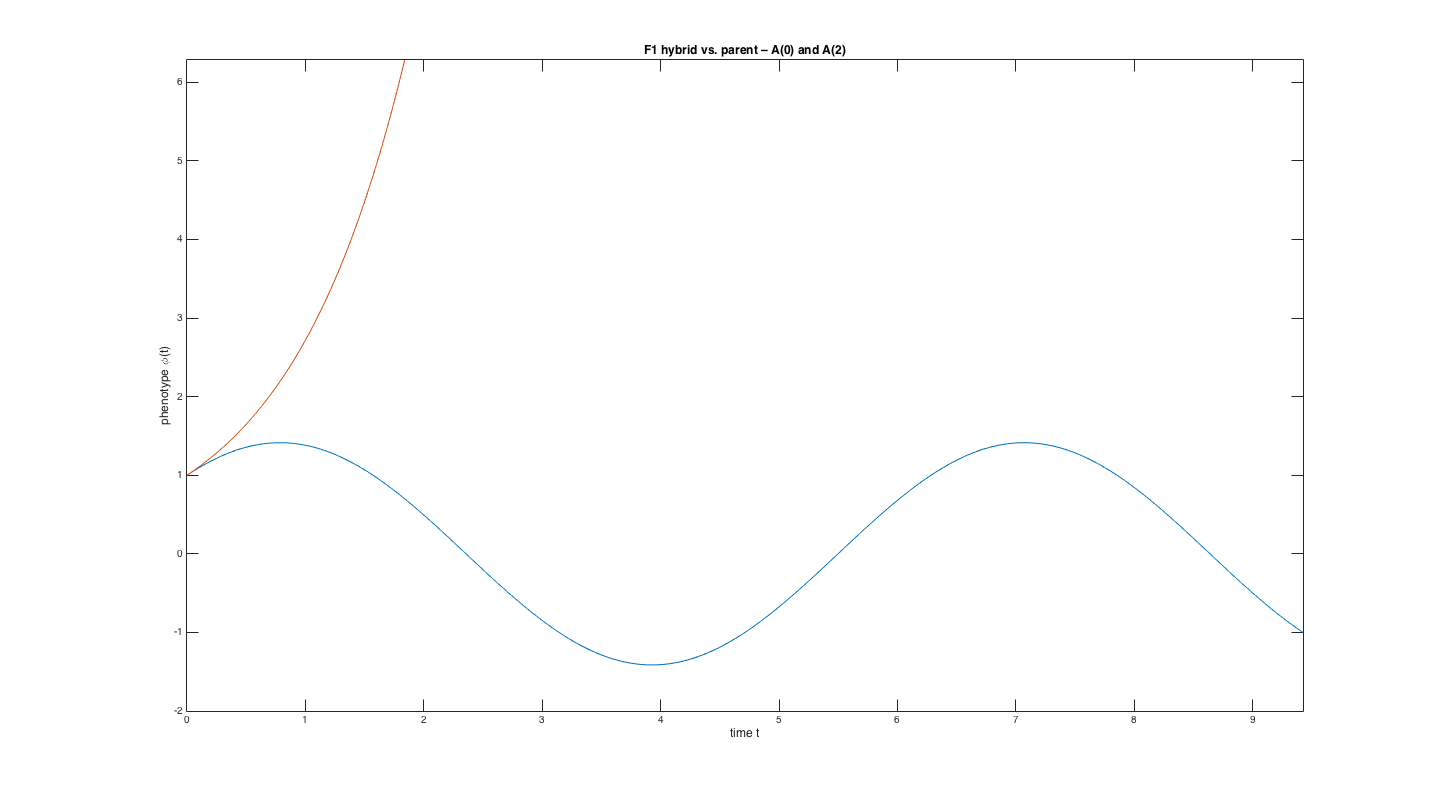
\includegraphics[width=0.5\textwidth, height=0.25\paperheight]{expF1}
        \caption{F1 hybrid (orange) and parental (blue) phenotypic oscillator dynamics for an $A(0)$ by $A(2)$ cross. The hybrid fails to oscillate and exhibits qualitatively different dynamics.}
      \end{figure}
 %     \begin{example}[F1 Reproductive Incompatibility in an Oscillating Gene Network]
 %       DMI examples...
 %       \begin{figure}[H]
 %         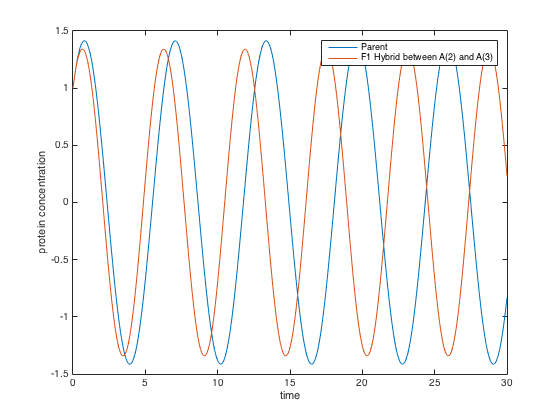
\includegraphics[width=0.5\textwidth]{A2_A3_osci_F1_hyb}
 %       \end{figure}
 %     \end{example}

      \begin{example}[Hybrid Incompatibility in an Oscillating Gene Network]

        Here we compare the phenotypes for F2 hybrids formed by crossing oscillators $A(2)$ with $A(2.01)$, $A(2.1)$, and $A(2.5)$ ($B$ and $C$ are the same as above). Each $A$ has is phenotypically identical ($\phi(t) = \sin(t) + \cos(t)$), however some of the hybrids exhibit markedly different dynamics. These differences tend to increase with time, quadratically ($x^{2}$) in F2s, and quartically ($x^{4}$) in F1s. 

%        \begin{align*}
 %         A(2) = \begin{bmatrix} 2 & -1 \\ 5 & -2 \end{bmatrix} &\qquad A(2.01) = \begin{bmatrix} 1.9901 & -0.9901 \\ 5.0101 & -1.9901 \end{bmatrix} \\
  %          A(2.1) = \begin{bmatrix} 1.9091 & -0.9091 \\ 5.1091 & -1.9091 \end{bmatrix} &\qquad A(2.5) = \begin{bmatrix} 1.6667 & -0.6667 \\ 5.6667 & -1.6667 \end{bmatrix}
   %     \end{align*} 

        \begin{alignat*}{2}
          A(2) &= \left[\begin{array}{cc} 2 & -1 \\[6pt] 5 & -2 \end{array}\right] &&\qquad A(2.01) = \left[\begin{array}{cc} 2 -\frac{1}{101} & -1 + \frac{1}{101} \\[6pt] 5 + \frac{1}{99} & -2 + \frac{1}{101} \end{array}\right] \\
            A(2.1) &= \left[\begin{array}{cc} 2 - \frac{1}{11} & -1 + \frac{1}{11} \\[6pt] 5 + \frac{6}{55} & -2 + \frac{1}{11} \end{array}\right] &&\qquad A(2.5) = \left[\begin{array}{cc} 2 - \frac{1}{3} & -1 + \frac{1}{3} \\[6pt] 5 + \frac{2}{3} & -2 + \frac{1}{3} \end{array}\right]
        \end{alignat*}
        F1 gene regulatory networks are formed by averaging the two parental $A(\tau)$ matrices; F2s are formed by first recombining parental matrices followed by an averaging. 
  %      \begin{figure}[H]
  %        \begin{tabular}{cc}
  %          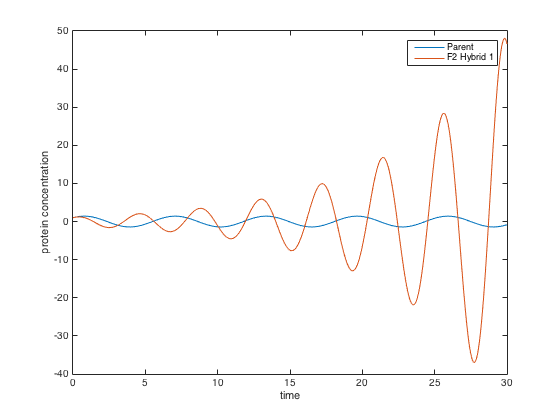
\includegraphics[width=0.2\textwidth]{A2_A3_osci_F2_hyb_1}
  %          & 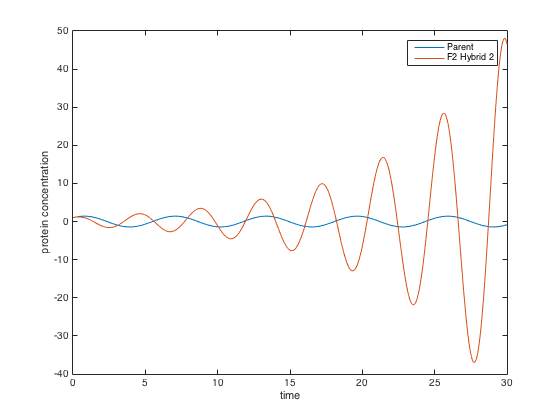
\includegraphics[width=0.2\textwidth]{A2_A3_osci_F2_hyb_2}
  %         \\ 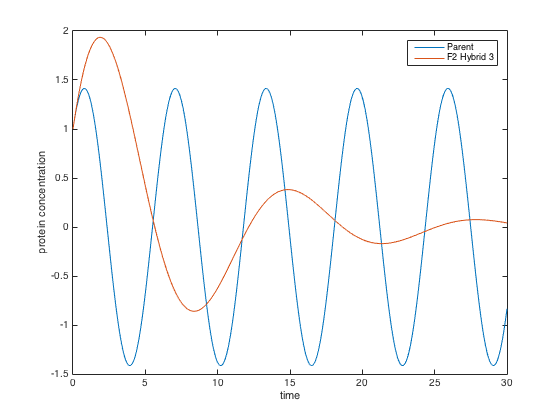
\includegraphics[width=0.2\textwidth]{A2_A3_osci_F2_hyb_3}
  %          & 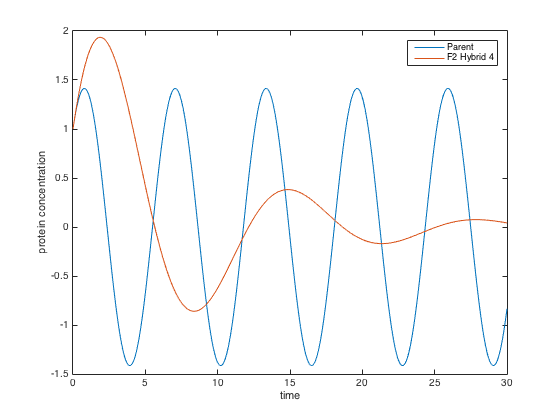
\includegraphics[width=0.2\textwidth]{A2_A3_osci_F2_hyb_4}
  %          \\ 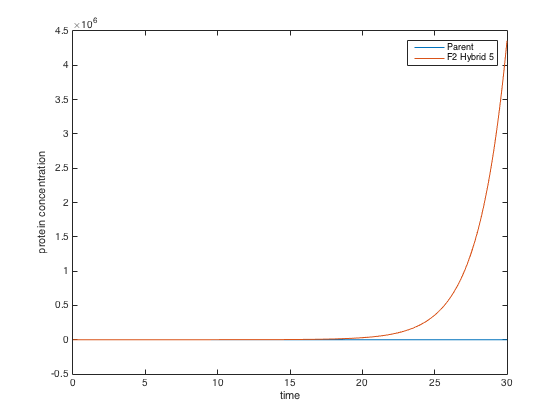
\includegraphics[width=0.2\textwidth]{A2_A3_osci_F2_hyb_5}
  %          & 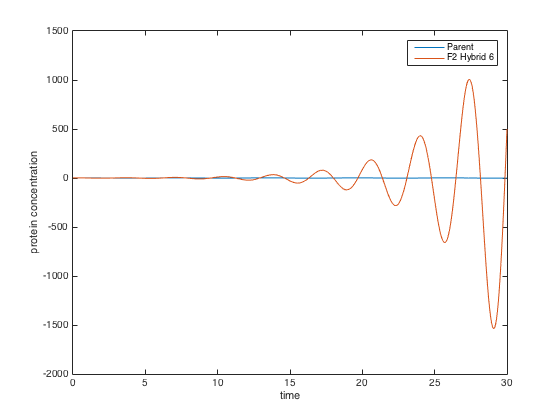
\includegraphics[width=0.2\textwidth]{A2_A3_osci_F2_hyb_6}
  %        \end{tabular}
  %      \end{figure}

  %    \begin{figure}[H]
  %      \centering
  %      \includegraphics[width=0.5\textwidth]{A2_A2-1_F2s}
  %      \caption{F2s from $A(2)$ and $A(2.1)$.}
  %    \end{figure}
  %      \begin{figure}[H]
  %        \begin{tabular}{cc}
  %        \includegraphics[width=0.5\textwidth]{F2s-small} \\
  %        \includegraphics[width=0.5\textwidth]{F2s} \\
  %        \includegraphics[width=0.5\textwidth]{F2s-large}
  %        \end{tabular}
  %        \caption{F2s from $A(2)$ and $A(2.1)$.}
  %      \end{figure}
        \begin{figure}[H]
          \centering
          \begin{tabular}{cc}
            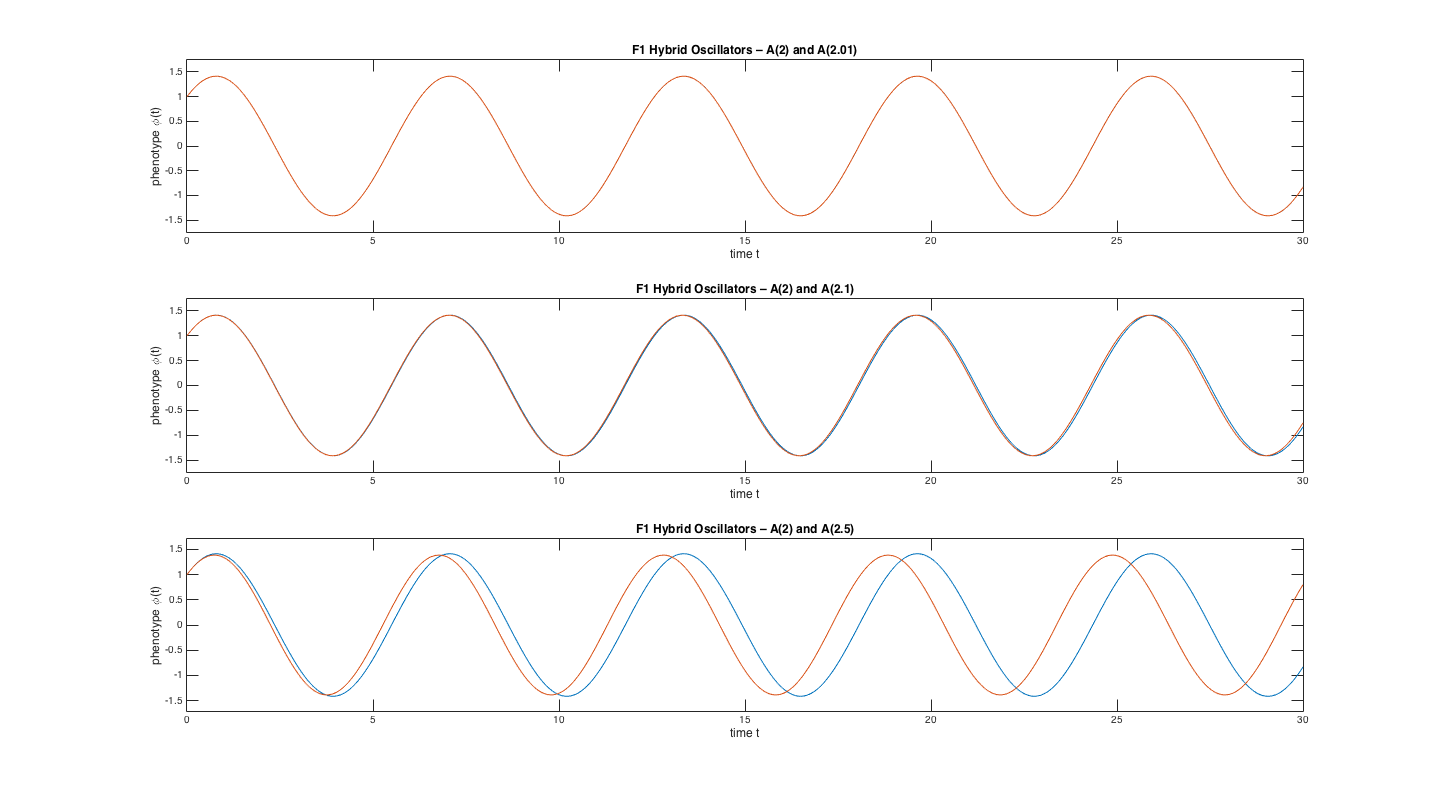
\includegraphics[width=0.5\textwidth, height=0.25\paperheight]{F1_comparison} & 
            \includegraphics[width=0.5\textwidth, height=0.25\paperheight]{F2_comparison}
          \end{tabular}
          \caption{F1 (left) and F2 (right) hybrids crossing $A(2)$ with $A(2.01)$ (top), $A(2.1)$ (middle), and $A(2.5)$ (bottom).
          Note the difference in scale on the $y$-axis. F2 hybrids display more phenotypic divergence than F1s, on average. Further, some F2s completely fail to oscillate, as seen in an $A(2.5)$ F2 (light blue).}
        \end{figure}
    \end{example}
      \begin{example}[Not all Networks can Host Incompatibilities]
        convex sets cant have DMIs

        \begin{align*}
          h(t) = 2 e^{- \theta t}
        \end{align*}
        Any non-minimal system with rows summing to $\theta$ is PI. Further, these systems are closed under averaging (mating) and row swapping (meiosis), leaving all hybrids optimally fit. The set of gene matrices is affine and therefore convex.  
      \end{example}

  \section*{Additionl Examples}

    \subsection*{Metabolic Network}
  \begin{align*}
    \dot{x}(t) &= \begin{bmatrix} 0 & 1 & 0 & -1 \\ 0 & 0 & -1 & -1 \\ -1 & 1 & 0 & 0 \\ 0 & 0 & 0 & 0 \end{bmatrix} \begin{bmatrix} \text{GAL3} \\ \text{GAL4} \\ \text{GAL80} \\ \text{MIG1} \end{bmatrix}(t) \\ &+ \begin{bmatrix} 1 & 0 & 0 \\ 0 & 0 & 1 \\ 0 & 0 & 0 \\ 0 & 1 & 1 \end{bmatrix} \begin{bmatrix} \text{galactose} \\ \text{glucose} \\ \text{BTM} \end{bmatrix}(t) \\
        y(t) &= \begin{bmatrix} 0 & 1 & 0 & -1 \end{bmatrix} \vec{x}(t)
    \end{align*}
    \begin{align*}
      H(z) &= \begin{bmatrix} 1 \\ z^{2} + z + 1 \\ z + 1 \end{bmatrix} \frac{1}{z^{3} + z -1}
    \end{align*}

    \begin{align*}
      CV &= C \\
      VB &= B \\
      V :&= \begin{bmatrix} 1 & 0 & a & 0 \\ 0 & 1 & 0 & 0 \\ 0 & 0 & b & 0 \\ 0 & 0 & 0 & 1 \end{bmatrix} , V^{-1} = \begin{bmatrix} 1 & 0 & \frac{-a}{b} & 0 \\ 0 & 1 & 0 & 0 \\ 0 & 0 & \frac{1}{b} & 0 \\ 0 & 0 & 0 & 1\end{bmatrix} \\
        A(a,b) :&= VAV^{-1} = \begin{bmatrix} -a & a+1 & \frac{a^{2}}{b} & -1 \\ 0 & 0 & \frac{-1}{b} & -1 \\ -b & b & a & 0 \\ 0 & 0 & 0 & 0 \end{bmatrix}
    \end{align*}
    The GAL regulatory network in \emph{S. cerevisiae} is modelled here. The activating transcription factor GAL4, which is regulated by the presence of galactose and two other TFs, binds to the promoter region of the GAL regulon -- a cluster of genes regulated by the same promoter encoding 3 enzymes (GAL1, GAL7, and GAL10), for the metabolism of the sugar galactose. The repressing transcription factor MIG1, which is activated by the presence of glucose and other proteins omitted here, also binds to the regulon, preventing the expression of the galactose metabolizing enzymes. This network is one of the most studied gene regulatory networks in yeast, and experiments have already demonstrated significant transcriptional variation among different species and genuses of yeast.

    In the present model, the $A$ matrix encodes the interactions among GAL3, GAL4, GAL80, and MIG1. $B$ interprets the input: the quantity of glucose, galactose, and the basal transcription (BTM) rates impact of TF concentrations. $C$ represents the promoter region of the GAL regulon and is the sum of the influence of GAL4 (activating) and MIG1 (repressing).

    $A(a,b)$ represent alternative network structures that produce identical outputs, with identical input and output transformations -- meaning the regulatory contributions of the sugars and the basasl machinery, as well as the promoter of the GAL regulon are held constant. These interactions may be realized in nature, if the regulatory differences predicted by $A(a,b)$ are biologically/mutationally realizable. Mutations influencing the interactions between GAL4 and GAL80 have been experimentally demonstrated \citep{li2010alterations}.

    \subsection*{Gap Gene Network}

    \section*{Discussion}
      \plr{mention $B$ part of genetic architecture}

      \jss{Discussion guidelines:
        \begin{itemize}
        \item Why is this important/useful?
        \item What are the assumptions and shortcomings of the research?
        \item Compare to other studies in the literature. 
        \item Future directions. 
        \item Wild speculations?
        \item Conclusion and overall impact. 
      \end{itemize}}

  The complexity of biological systems has limited our understanding of their function and evolution. Above we outline an approach, a first step, towards untangling this complexity in reference to function and evolution. This methodology borrows successfully applied tools from engineering and aims to synthesize these with the concepts and tools of molecular and evolutionary biology. 
  
  Theoretical models in evolution and population genetics often lack the molecular details of physiology or of the genotype-phenotype map. Here, we offer a tractable and simple model which includes these missing features. Further, we provide, in clear mathematical language, an analytical description of phenomena hitherto only discussed verbally and conceptualy (phenogenetic drift \citep{weiss2000phenogenetic}, developmental systems drift \citep{true2001developmental}, biological degeneracy \citep{edelman2001degeneracy}, \emph{etc.}). The tractability and relative simplicity of this exposition enables the interested biologist to work out by hand, if desired, the dynamics of a genetic system, as well as perturbations to the system -- an attribute not likely to be found in less tractable models and simulations.

  We have suggested an interpretation of system identification: to see it as an evolutionarily neutral manifold, and not simply a computational nuissance. We have demonstrated a method to analytically determine the set of all phenotypically invarint gene networks; by a simple change of coordinates in the minimal configuration, or more generally by applying the Kalman decomposition in higher dimensions. Further, we emphasize that evolution proceeds through this high dimensional space as stochastic coordinate transformation, constrained by sexual reproduction and selection. This set is explored over evolutionary time when phenotype is conserved, and can lead to a diverse set of consequences, including the accumulation of Dobzhansky-Muller incompatibilities. We emphasize that these incompatibilities are a consequence of recombining different, yet functionally equivalent, mechanisms. We also suggest that gene networks may not always use their components parsimoniously as network size tends to ratchet up in the absence of strong selection against extra parts. Although unexplored presently, this phenomena may lead to insights on evolvability and developmental innovation. Lastly, we show that hybrid gene networks break down as function of genetic distance, and may, in part, explain broad patterns of reproductive isolation among diverse phyla \citep{roux2016shedding}.

  As Richard Levins opined, models in population biology face a tradeoff among precision, realism, and generality \citep{levins1966strategy}. As Levins expects, any tractable and general model, such as the present one under discussion, will have limitations. Most notable is linearity. It is often stated that life is not linear. This is often true, however, many of the ideas developed here should be generalizable to nonlinear cases (multilinear systems, say). Futher, we see this as a necessary first step in the direction of more life-like nonlinear evolutionary systems theory. Depending on an actual biological system's particularities, its (potential) nonlinearity, may buffer or exacerbate effects elucidated in this paper, such as the aquisition of Dobzansky-Muller incompatibilities.

  This theoretical framework can easily be applied to other interesting questions in evolutionary biology not tackled presently: such as the evolution of linkage, the necessity of network complexity (does evolution tend towards Rube Goldberg or \jss{parsimonious} network organization?), evolvability, structure/function inference, and intrapopulation context dependency of mutational effects, as well as many others.

  \jss{literature comparison:}

  Over the last several years, several different computational approaches have been applied to study reproductive incompatibility and speciation. \citet{tulchinsky} simulated the evolution of a transcription factor and its binding site using a thermodynamic model. Their simulations suggest that the language by which a transcription factor recognizes its binding site can change, and potentially lead to hybird incomaptibility when allopatric populations employ divergent readout languages. This study, despite looking at gene regulation, does not analyze overall gene network architecture -- as we do here -- it only looks at the expression level of a single gene. Furthermore, they report reproducitve isolation primarily following direcitonal selection for a change in expression levels in each allopatric population; the evidecne for reproductive isolation following balancing selection is much weaker. Johnson and Porter 2000 did not observe any hybrid fitness declines under stabilizing selection -- only under directional selection. 
  Khatari et al, Tulchinsky et al, and Porter et al, all study hybrid incompatibility from a transcription factor/binding site interaction perspective, not from an overal network architecture perspective. Palmer and Feldman only see hybrid incompatibility in constant environments if the parental populations are relatively poorly adapted initially. Otherwise hybrids between two allopatric populations have fairly high fitnesses.  

\section*{Acknowledgements}
We would like to thank Sergey Nuzhdin, Stevan Arnold, Erik Lundgren, and Hossein Asgharian for valuable discussion.

\bibliographystyle{plainnat}
\bibliography{krefs}
%\end{multicols}

\normalsize
\appendix

\section{Genetic drift with a multivariate trait}
\label{ss:quant_gen}

For completeness, we provide a brief argument of how the population mean
moves under genetic drift
with a quantitative genetics model,
as in \citet{lande1981models} or \citet{hansen1996translating}.
These ignore details of the underlying genetic basis,
but developing a more accurate model is beyond the scope of this paper.

\paragraph{Completing the square}
First note that 
\begin{align*}
    (x-y)^T A (x-y)
    &=
    x^T A \left( x - 2y \right) + y^T A y ,
\end{align*}
and so
\begin{align*}
    (x-y)^T A (x-y) + x^T B x
    &=
    x^T (A + B) \left( x - 2 (A + B)^{-1} A y \right) + y^T A y \\
    &=
    \left( x - (A + B)^{-1} A y \right)^T
    (A + B)
    \left( x - (A + B)^{-1} A y \right)
    + \text{(terms that don't depend on $x$)} .
\end{align*}
Therefore, if $f(x;\Sigma,y)$ is the density of a Gaussian with mean $y$ and covariance matrix $\Sigma$
then substituting $A=\Sigma^{-1}$ and $B=U^{-1}$ above,
\begin{align*}
    \frac{ f(x;\Sigma,y) f(x;U,0) }{\int_x f(z;\Sigma,y) f(z;U,0) dz}
    &=
    f(x; (\Sigma^{-1} + U^{-1})^{-1}, (\Sigma^{-1}+U^{-1})^{-1} \Sigma^{-1} y) .
\end{align*}

Now suppose that the population is distributed in genotype space
as a Gaussian with covariance matrix $\Sigma$ and mean $y$.
Selection has the effect of multiplying this density by the fitness function and renormalizing,
so that if expected fitness of $x$ is proportional to $f(x;U,z)$
then the above argument shows that the next generation will be sampled from a Gaussian distribution
with covariance matrix $(\Sigma^{-1} + U^{-1})^{-1}$ 
and mean $z + (\Sigma^{-1}+U^{-1})^{-1} \Sigma^{-1} (y-z)$
Taking a sample of size $N$ to construct the next generation 
will produce something close to this but with a slightly (stochastically) deviating mean.
The next generation's mean is drawn from a Gaussian distribution with mean
with covariance matrix $(\Sigma^{-1} + U^{-1})^{-1}/N$ 
and mean $z + (\Sigma^{-1}+U^{-1})^{-1} \Sigma^{-1} (y-z)$.

Roughly, what is this doing?
Suppose that the population mean differs from the optimum by $\epsilon$,
that $\Sigma = \sigma^2 I$ and $U = s I$.
Then the population mean gets closer to the optimum on average, moving to
$\epsilon/(1 + \sigma^2/s)$
and adds noise of size $\sqrt{s} \sigma/\sqrt{N \sigma^2 + N s}$.
At equilibrium, these two movements will be of the same order,
so that $\epsilon$ is of order $(\sigma/\sqrt{N}) \sqrt{1+\sigma^2/s}$.


\section{Differentiating the fitness function}

Suppose that $\rho(t) \ge 0$ is a weighting function on $[0,\infty)$
so that fitness is a function of $L^2(\rho)$ distance of the impulse response from optimal.
With $A_0$ a representative of the optimal set:
\begin{equation}
    \begin{aligned}
        D(A) 
        &:= 
        \int_0^\infty \rho(t) \left| h_A(t) - h_{A_0}(t) \right|^2 dt \\
        &:= 
        \int_0^\infty \rho(t) \left| C e^{At} B - C e^{A_0 t} B \right|^2 dt \\
        &= 
        \int_0^\infty \rho(t) \left| C \left( e^{At} - e^{A_0 t} \right) B \right|^2 dt \\
        &= 
        \int_0^\infty \rho(t) C \left( e^{At} - e^{A_0 t} \right) B B^T \left( e^{At} - e^{A_0 t} \right)^T C^T dt
    \end{aligned}
\end{equation}
How does this change with $A$?
Since
\begin{equation}
  \begin{aligned}
      \frac{d}{du} e^{(A+uZ)t} \vert_{u=0}
      &=
      \int_0^t e^{As} Z e^{A(t-s)} ds, 
  \end{aligned}
\end{equation}
we have that
\begin{equation}
  \begin{aligned}
      \frac{d}{du} D(A+uZ)\vert_{u=0}
      &=
        2 \int_0^\infty \rho(t) C \left( \int_0^t e^{As} Z e^{A(t-s)} ds \right) B B^T \left( e^{At} - e^{A_0 t} \right)^T C^T dt \\
      &=
        2 \int_0^\infty \rho(t) C \left( \int_0^t e^{As} Z e^{A(t-s)} ds \right) B \left( h_A(t) - h_{A_0}(t) \right)^T dt 
  \end{aligned}
\end{equation}
and, by differentiating this and supposing that $A$ is on the optimal set,
i.e., $h_A(t)=h_{A_0}(t)$, (so wolog $A=A_0$):
\begin{equation}
  \begin{aligned}
      \calH(Y,Z) &:= \frac{1}{2} \frac{d}{du} \frac{d}{dv} D(A_0+uY+vZ)\vert_{u=v=0} \\
      &=
        \int_0^\infty \rho(t) C 
        \left( \int_0^t e^{A_0 s} Y e^{A_0 (t-s)} ds \right) 
        B B^T 
        \left( \int_0^t e^{A_0 s} Z e^{A_0 (t-s)} ds \right)^T
        C^T dt  .
  \end{aligned}
\end{equation}
Here $\calH$ is the quadratic form underlying the Hamiltonian.
By defining $\Delta_{ij}$ to be the matrix with a 1 in the $(i,j)$th slot
and 0 elsewhere,
the coefficients of the quadratic form is
\begin{equation}
    \begin{aligned}
        H_{ij, k\ell}(A)
        &:=
        \calH(\Delta_{ij}, \Delta_{k\ell}) .
    \end{aligned}
\end{equation}

We could use this to compute the gradient of $D$,
or to get the quadratic approximation to $D$ near the optimal set.
To do so, it'd be nice to have a way to compute the inner integral above.
Suppose that we can diagonalize $A = U \Lambda U^{-1}$.
Then
\begin{equation} \label{eqn:exp_deriv}
  \begin{aligned}
      \int_0^t e^{As} Z e^{A(t-s)} ds 
      &=
      \int_0^t U e^{\Lambda s} U^{-1} Z U e^{\Lambda (t-s)} U^{-1} ds 
  \end{aligned}
\end{equation}
Now, notice that
\begin{equation}
  \begin{aligned}
      \int_0^t e^{s \lambda_i} e^{(t-s) \lambda_j} ds
      &=
      \frac{ e^{t \lambda_i} - e^{t \lambda_j} }{ \lambda_i - \lambda_j } .
  \end{aligned}
\end{equation}
Therefore, 
defining
\begin{equation}
    X_{ij}(t,Z) = \left( U^{-1} Z U \right)_{ij}
      \frac{ e^{t \lambda_i} - e^{t \lambda_j} }{ \lambda_i - \lambda_j } 
\end{equation}
moving the $U$ and $U^{-1}$ outside the integral and integrating we get that
\begin{equation}
  \begin{aligned}
      \int_0^t e^{As} Z e^{A(t-s)} ds 
      &=
      U X(t,Z) U^{-1} .
  \end{aligned}
\end{equation}

Following on from above, we see that if $Z=\Delta_{k \ell}$, then
\begin{equation}
  \begin{aligned}
      X_{ij}^{k\ell}(t) = 
      \frac{ e^{t \lambda_i} - e^{t \lambda_j} }{ \lambda_i - \lambda_j } 
      (U^{-1})_{\cdot k} U_{\ell \cdot},
  \end{aligned}
\end{equation}
where $U_{k \cdot}$ is the $k$th row of $U$,
and so
\begin{equation}
    \begin{aligned}
        H_{ij, k\ell}(A)
        &=
        \int_0^\infty
            \rho(t) C U X^{ij}(t) U^{-1} B B^T (U^{-1})^T X^{k\ell}(t)^T U^T C^T
        dt .
    \end{aligned}
\end{equation}
This implies that
\begin{equation}
    \begin{aligned}
        D(A_0+\epsilon Z)
        &\approx \epsilon^2\sum_{ijk\ell} H^{ij,k\ell} Z_{ij} Z_{k\ell} 
    \end{aligned}
\end{equation}
and so
\begin{equation}
    \begin{aligned}
        D(A_0+\epsilon Z)
        &\approx \epsilon^2\sum_{ijk\ell} H^{ij,k\ell} Z_{ij} Z_{k\ell} 
    \end{aligned}
\end{equation}

By section \ref{ss:quant_gen},
if we set $\Sigma=\sigma^2 I$ and $U=H$,
then a population at $A_0+Z$ experiences a restoring force of strength
$(I + \sigma^2 H^{-1})^{-1} Z$ (treating $Z$ as a vector and $H$ as an operator on these).
If $\sigma^2$ is small compared to $H^{-1}$
then this is approximately $-\sigma^2 H^{-1} Z$.
This suggests that the population mean follows an Ornstein-Uhlenbeck process,
as described (in different terms) in \citet{hansen1996translating}.

\end{document}
